% comment out for student version
\ifdefined\Student\relax\else\def\Teacher{}\fi

\documentclass[12pt]{article}

\title{Local Variables}
\author{Chris Mayfield}
\date{Summer 2021}

%\ProvidesPackage{cspogil}

% fonts
\usepackage[utf8]{inputenc}
\usepackage[T1]{fontenc}
\usepackage{mathpazo}

% spacing
\usepackage[margin=2cm]{geometry}
\renewcommand{\arraystretch}{1.4}
\setlength{\parindent}{0pt}

% orphans and widows
\clubpenalty=10000
\widowpenalty=10000
\pagestyle{empty}

% figures and tables
\usepackage{graphicx}
\usepackage{multicol}
\usepackage{tabularx}
\usepackage{wrapfig}

% fixed-width columns
\usepackage{array}
\newcolumntype{L}[1]{>{\raggedright\let\newline\\\arraybackslash\hspace{0pt}}m{#1}}
\newcolumntype{C}[1]{>{\centering\let\newline\\\arraybackslash\hspace{0pt}}m{#1}}
\newcolumntype{R}[1]{>{\raggedleft\let\newline\\\arraybackslash\hspace{0pt}}m{#1}}

% include paths
\makeatletter
\def\input@path{{Models/}{../../Models/}}
\graphicspath{{Models/}{../../Models/}}
\makeatother

% colors
\usepackage[svgnames,table]{xcolor}
\definecolor{bgcolor}{HTML}{FAFAFA}
\definecolor{comment}{HTML}{007C00}
\definecolor{keyword}{HTML}{0000FF}
\definecolor{strings}{HTML}{B20000}

% table headers
\newcommand{\tr}{\bf\cellcolor{Yellow!10}}

% syntax highlighting
\usepackage{textcomp}
\usepackage{listings}
\lstset{
    basicstyle=\ttfamily\color{black},
    backgroundcolor=\color{bgcolor},
    numberstyle=\scriptsize\color{comment},
    commentstyle=\color{comment},
    keywordstyle=\color{keyword},
    stringstyle=\color{strings},
    columns=fullflexible,
    keepspaces=true,
    showlines=true,
    showstringspaces=false,
    upquote=true
}

% code environments
\newcommand{\java}[1]{\lstinline[language=java]{#1}}%[
\lstnewenvironment{javalst}{\lstset{language=java,backgroundcolor=}}{}
\lstnewenvironment{javabox}{\lstset{language=java,frame=single,numbers=left}\quote}{\endquote}

% PDF properties
\usepackage[pdftex]{hyperref}
\urlstyle{same}
\makeatletter
\hypersetup{
  pdftitle={\@title},
  pdfauthor={\@author},
  pdfsubject={\@date},
  pdfkeywords={},
  bookmarksopen=false,
  colorlinks=true,
  citecolor=black,
  filecolor=black,
  linkcolor=black,
  urlcolor=blue
}
\makeatother

% titles
\makeatletter
\renewcommand{\maketitle}{\begin{center}\LARGE\@title\end{center}}
\makeatother

% boxes [optional height]
\newcommand{\emptybox}[1][10em]{
\vspace{1em}
\begin{tabularx}{\linewidth}{|X|}
\hline\\[#1]\hline
\end{tabularx}}

% models
\newcommand{\model}[1]{\section{#1}\nopagebreak}
\renewcommand{\thesection}{Model~\arabic{section}}

% questions
\newcommand{\quest}[1]{\subsection*{Questions~ (#1)}}
\newcounter{question}
\newcommand{\Q}{\vspace{1em}\refstepcounter{question}\arabic{question}.~ }
\renewcommand{\thequestion}{\#\arabic{question}}

% sub-question lists
\usepackage{enumitem}
\setenumerate[1]{label=\alph*)}
\setlist{itemsep=1em,after=\vspace{1ex}}

% inline answers
\definecolor{answers}{HTML}{C0C0C0}
\newcommand{\ans}[1]{%
\ifdefined\Student
    \leavevmode\phantom{~~\textcolor{answers}{#1}}
\else
    ~~\textcolor{answers}{#1}
\fi}

% longer answers [optional height]
\newsavebox{\ansbox}
\newenvironment{answer}[1][4em]{
\nopagebreak
\begin{lrbox}{\ansbox}
\begin{minipage}[t][#1]{\linewidth}
\color{answers}
}{
\end{minipage}
\end{lrbox}
\ifdefined\Student
    \phantom{\usebox{\ansbox}}%
\else
    \usebox{\ansbox}%
\fi}


\begin{document}

\maketitle

%\model{Local Variables}

Consider the following example.
The memory diagram shows the state of the program just before \java{printResult} returns for the second time:

\medskip
\begin{javalst}
public static void printResult(int qty, double amt) {
    System.out.printf("%d for $%.2f\n", qty, amt);
}

public static void main(String[] args) {
    int count = 3;
    double price = 9.99;
    char grade = 'A';
    boolean okay = true;
    printResult(count, price);
    count++;
    price *= 2;
    okay = !okay;
    printResult(count, price);
}
\end{javalst}

\bigskip
The output of the program is:

\begin{verbatim}
3 for $9.99
4 for $19.98
\end{verbatim}

\vspace{-26em}
\hfill 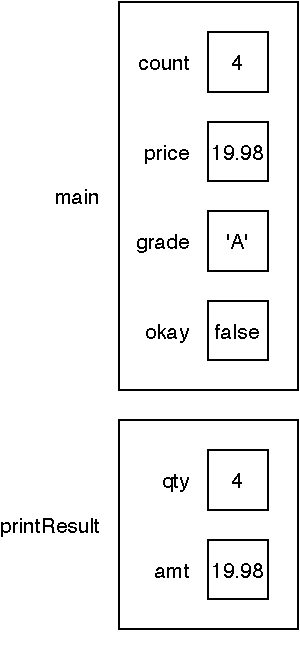
\includegraphics{local-diagram.pdf}
\hspace{2em} \null


\quest{15 min}


\Q How many variables are declared \ldots

\begin{multicols}{2}
\begin{enumerate}
\item in \java{main}? \ans[3em]{4}
\item in \java{printResult}? \ans[3em]{2}
\end{enumerate}
\end{multicols}


\Q How many times is each variable assigned?

\begin{multicols}{2}
\begin{enumerate}
\item \java{count} \ans[3em]{2} \note{including ++}
\item \java{price} \ans[3em]{2}
\item \java{grade} \ans[3em]{1}
\item \java{okay}  \ans[3em]{2}
\item \java{qty}   \ans[3em]{2} \note{two method calls}
\item \java{amt}   \ans[3em]{2}
\end{enumerate}
\end{multicols}


\Q Is there a small box for each declaration or each assignment? Justify your answer.

\begin{answer}[3em]
Each declaration; otherwise there would be more than four boxes in \java{main}.
\end{answer}


\Q What do the six small boxes in the memory diagram represent?

\begin{answer}[3em]
The contents of memory for each of the variables.
\end{answer}


\Q What do the two large boxes in the memory diagram represent?

\begin{answer}[3em]
The stack frames for each method, showing which variables are defined.
\end{answer}


\Q \label{key1}
Why does the diagram indicate that \java{count} is \java{4} and \java{price} is \java{19.98}, even though the source code says that \java{count = 3} and \java{price = 9.99}?

\begin{answer}[3em]
The variables were modified later in the program.
The diagram shows the state of memory near the end.
\end{answer}


\Q Based on the source code:

\begin{enumerate}
\item Which method is defined first? \ans[8em]{printResult}
\item Which method is executed first? \ans[8em]{main}
\end{enumerate}


%\Q In what order are the methods shown in the memory diagram? Why?
%
%\begin{answer}[3em]
%Methods are shown in the order of execution, because the diagram represents the state of memory over time.
%\end{answer}


\Q Copy the contents of \textit{LocalVariables.java} into \href{https://cscircles.cemc.uwaterloo.ca/java_visualize/#code=public+class+ClassNameHere+%7B%0A++++public+static+void+main(String%5B%5D+args)+%7B%0A++++++++%0A++++%7D%0A%7D&mode=edit&showStringsAsObjects=1}{Java Visualizer}.
Click the ``Visualize execution'' button, and then click ``Forward $>$'' multiple times to see the code run.

\begin{enumerate}

\item What does the diagram look like on Step 11 of 19, just before \java{count++} executes?

\begin{answer}[3em]
There is only one frame (for \java{main}) with four variables:
count=3, price=9.99, grade=\chr{A}, and okay=true.
\end{answer}

\item Why is there no frame for the \java{printResult} method on Step 11 of 19?

\begin{answer}[3em]
The method is not currently active; it returned during the previous step.
\end{answer}

\item Run the program to Step 17 of 19, just before \java{printResult} returns for the second time.
What differences do you notice between the diagram on the previous page and the one on Java Visualizer?

\begin{answer}[6em]
Answers might include:
\bull All boxes (variables and frames) have four sides in the activity.
\bull The frames are drawn in opposite order (top-down vs bottom-up).
\bull Java Visualizer labels the frames on top and shows the line number.
\bull Java Visualizer shows the method return values (even when \jans{void}).
\end{answer}

\end{enumerate}

\end{document}
